\subsection{Imaging}

Digital stereo vision in the end analyses digital images; this chapter introduces the basic concerns that affect reconstruction quality. Cameras are never ideal, and practical algorithms take lens imperfections into account (see e.g. opencv [? that net page about distortion]). Images are commonly taken with digital cameras that project a three-dimensional view from a single viewpoint to an image plane, and finally to a discrete grid of numerical values that describe light intensities.

Practical details, such as depth of field, camera sensor noise, aberrations and others are not considered, as they vary greatly depending on the used hardware and are out of scope of this work. It suffices to say that in a practical system the choice of good optics is a key to good quality reconstruction.

In addition to plain photographic cameras, reconstruction can be done using e.g. laser scanners or light field cameras. Those are not covered in this work.

\subsubsection{Pinhole camera}

A camera is in its simplest form modeled as a pinhole camera; an ideal thin lens that projects an image upside down on its film. Illustration given in image \ref{fig:pinhole-camera}. In computer vision, this projection is given as a $3 \times 4$ matrix, when homogenous coordinates \cite[?] are used. The pinhole model (or, perspective projection) states that the world point $(x, y, z)$ is projected to the image plane at $(u, v)$:

\begin{equation}
\begin{pmatrix}
u \\ v
\end{pmatrix}
=
\frac{f}{z} \begin{pmatrix}
x \\ y \\ z
\end{pmatrix}
\end{equation}


%\simplegfx{h}{0.9\textwidth}{pinhole-camera}
%{Pinhole camera principle. The box represents a camera; image is formed to the plane on its back.}

\subsubsection{Optics}

Construction of optical systems is well studied [?,?,?]. Actual camera lenses consist usually of not only a single glass element but many, especially in the case of zoom lenses [?]. In this work, the inner workings of these systems are ignored and equations assume a simple projective model.

The following equation applies for a thin lens while capturing sharp images:

\begin{equation}
	\frac{1}{a} + \frac{1}{b} = \frac{1}{f} \label{eq:focal}
\end{equation}

where f is the focal length, a is the distance between the lens and the film, and b is the distance between the lens and the imaged source. This is illustrated in figure TODO.

The focal length has a direct influence to field of view, as given in figure TODO. Longer focal length (long-focus lens, often referred to as telephoto lens) results to a more zoomed in picture, as opposed to a wide-angle lens. 

All practical optical systems (lenses) introduce some non-linear distortion that affects the performance of the ideal pinhole model.

Common distortions are the purely radial so-called barrel and pincushion distortions, where the magnification is a nonlinear function of image ray distance from the center of the lens.
Fisheye lenses are commonly known to have this kind of effect.
Tangential distortion is less common, particularly in great magnitudes, and is often ignored. Its cause is small misalignments in separate elements in a single optical system; lenses being offset from each other and not parallel to the image plane.

Wilson \cite{wilson2004anton} discusses optical systems' relation to depth of field, focus and distortions.

Perspective distortion something something viewer location. Normal TV is usually watched at the distance of twice the screen diagonal. At this location, the scene looks normal when taken with a normal lens. A wide-angle scene then looks normal when viewed at a nearer distance. \cite{wilson2004anton}

% 14:01:55 <naavis> Kai sillä yritetään emuloida sitä, että katsojan paikalta se leffan kuvakenttä vastais sitä että valkokankaan tilalla on ikkuna.

% TODO: custom tikz for exactly specified parameters in barrel/radial

%\simplefig{h}{%
%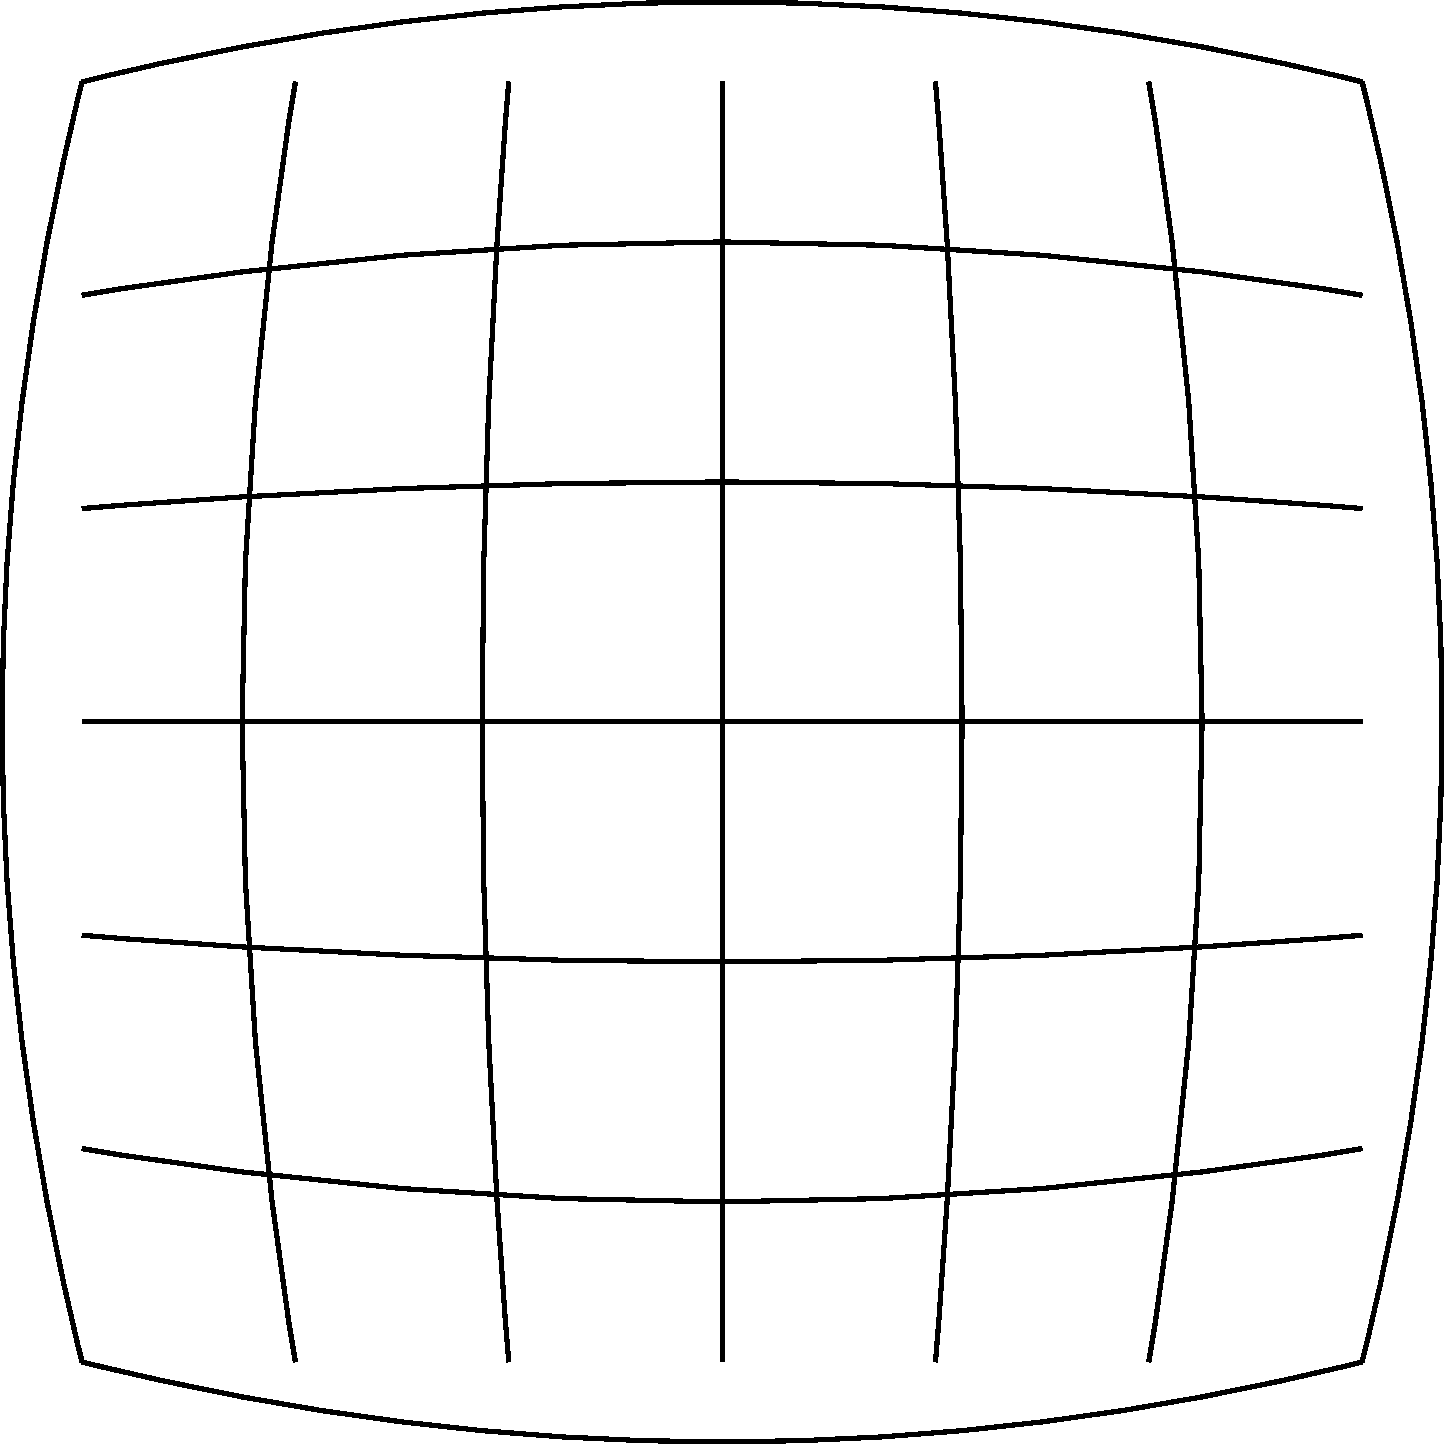
\includegraphics[width=0.3\textwidth]{gfx/barrel-distortion}
%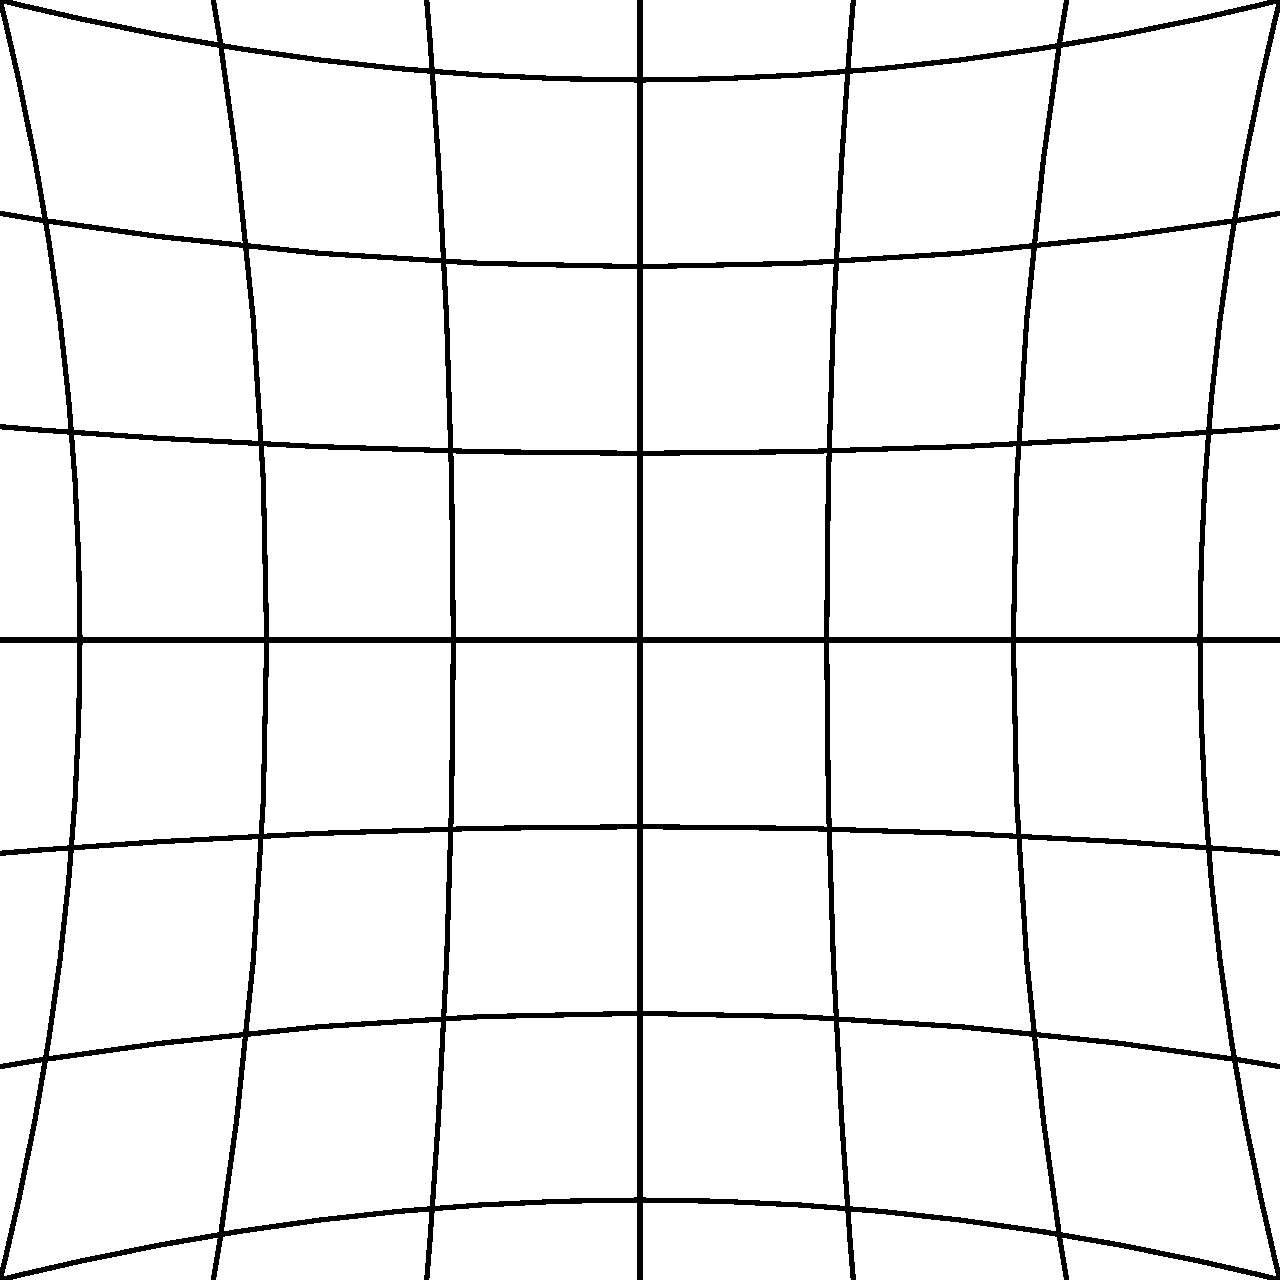
\includegraphics[width=0.3\textwidth]{gfx/pincushion-distortion}
%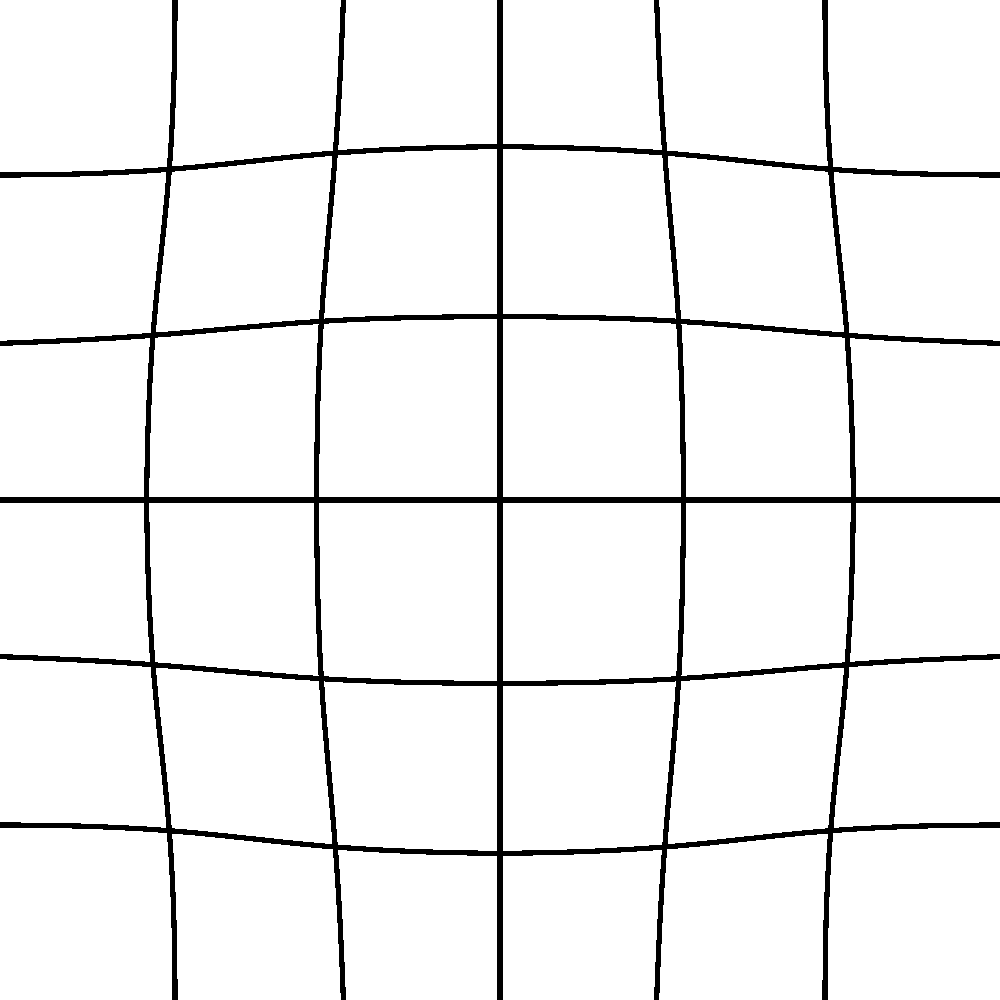
\includegraphics[width=0.3\textwidth]{gfx/mustache-distortion}
%}{fig:distortions}
%{Left to right: barrel, pincushion and mustache distortions, respectively.}

Distortion should be corrected in software, as the following stereo algorithms assume that the images are free of nonlinear errors, i.e. straight lines in the world should remain straight in 2D images after the projective transformation.
In particular, image rectification [X] won't work if this straightness does not remain; the assumption that similar features should be found on horizontal lines wouldn't hold on distorted images.

The radial correction used by the OpenCV library is

\begin{align}
	x_{corr} &= x(1 + k_1 r^2 + k_2 r^4 + k_3 r^6)\\
	y_{corr} &= y(1 + k_1 r^2 + k_2 r^4 + k_3 r^6)
\end{align}

Trucco and Verri \cite{trucco1998introductory} use only the two first coefficients. For tangential distortion, the formulas are

\begin{align}
x_{corr} &= x + (2 p_1 x y + p_2 (r^2 + 2 x^2))\\
y_{corr} &= y + (2 p_2 x y + p_1 (r^2 + 2 y^2))
\end{align}

where $x$ and $y$ are the original coordinates in the distorted image, $x_{corr}$ and $y_{corr}$ are the corrected ones, $k_1$, $k_2$, $k_3$, $p_1$ and $p_2$ are coefficients specific to the distortion, and $r$ equals to the distance to image center located at $(x_c,~y_c)$:

\begin{equation}
r = \sqrt{(x - x_c)^2 + (y - y_c)^2}
\end{equation}

TODO: example pic of a fisheyed image and undistorted one.

\subsubsection{Shutter}

In dynamic (i.e. moving) environments, the process of acquiring several images consecutively is an important thing to consider. When a group of cameras are capturing the same target, they should operate synchronously and grab images at same infinitesimally small points in time. In reality, there is error: the cameras do not work in perfect sync, and their sensors take some time to acquire an image.

CCD (Charge-coupled Device)

Global shutter

CMOS (Complementary Metal-Oxide Semiconductor)

Cheaper, rolling shutter: reading the pixels out happens linearly

Moreover, a CCD sensor should be used in place of a chaper CMOS sensor; CCDs incorporate a ``global hutter'', i.e. the whole sensor images the scene at once. A phenomenon called ``rolling shutter'' is common in CMOS sensors: the reading happens linearly, and moving objects get distorted.

Uniform lightning (lightness constancy or what)

Mechanical vs. electrical (varying ccd charge time)

Shutter vs frame rate. More discussed in the section \ref{subsec:video}. Shutter duration that exposes half of the frame time is common in professional motion pictures \cite{wilson2004anton}. While the shutter is closed, the film advances to next frame (in mechanical cameras). Blur makes the human mind think that the movement is smooth. When sampling for 3D reconstruction, the ideal shutter speed would be infinitesimally fast to reduce blur. Movement in between is then interpolated.

Flash visibility, short flash, flash shared to two frames

Image upside down on the sensor, curtain goes physically from top to bottom

Shutter lag (AE/AF even in manual mode maybe?); consistent or not?

Rieke-Zapp et al \cite{rieke2009evaluation} address several problems in camera calibration and imaging quality, e.g. mechanical problems blah blah

Polarization filter can be used to reduce specular highlights. [?] 

